\documentclass[12pt,a4paper,titlepage]{book}

\usepackage[lighttt]{lmodern}
\usepackage[T1]{fontenc}
\usepackage[utf8]{inputenc}
\usepackage[headheight=15.5pt]{geometry}
\usepackage{graphicx}
\usepackage[hidelinks]{hyperref}

% configurazione e macro per documento multilingua
\usepackage[english,italian]{babel}
\newcommand\eng[1]{\foreignlanguage{english}{#1}}
\newcommand\eeng[1]{\foreignlanguage{english}{\emph{#1}}}

% configurazione bibliografia e citazioni
\usepackage[autolang=hyphen,style=numeric-comp]{biblatex}
\addbibresource{tesi.bib}
\usepackage[autostyle,italian=quotes]{csquotes}

% personalizzazione testatine e relative marche
\usepackage{fancyhdr}
\pagestyle{fancy}
\renewcommand{\chaptermark}[1]{\markboth{\uppercase{\thechapter.~#1}}{}}
\renewcommand{\sectionmark}[1]{\markright{#1}}

% personalizzazione titoli di capitoli/sezioni
\usepackage{titlesec}
\titleformat{\chapter}[hang]{\Huge\bfseries}{\thechapter.}{1em}{}
\setlength{\parindent}{0pt}
\setlength{\parskip}{0.5\baselineskip plus1pt minus1pt}

% personalizzazione indice
\usepackage{tocloft}
\renewcommand{\cftdot}{}

% personalizzazione liste
\usepackage{enumitem}
\setlist{itemsep=0pt, topsep=1ex, parsep=1ex}

% personalizzazione didascalie figure
\usepackage[justification=centering]{caption}

\usepackage{lipsum} % cancellami

% ============================================================================

\begin{document}
\frontmatter
\pagestyle{plain}
\newgeometry{left=1cm,bottom=1.5cm,right=1cm,top=1cm}
\thispagestyle{empty}
\begin{center}
{\setlength{\parskip}{0pt}
\textsc{\Large Università Politecnica delle Marche}\par
\noindent\rule{\textwidth}{1pt}\par\vspace{2ex}
{\large\uppercase{facoltà di ingegneria}\par\vspace{1ex}
Corso di Laurea [Magistrale] in Ingegneria Informatica}\par\vspace{1cm}
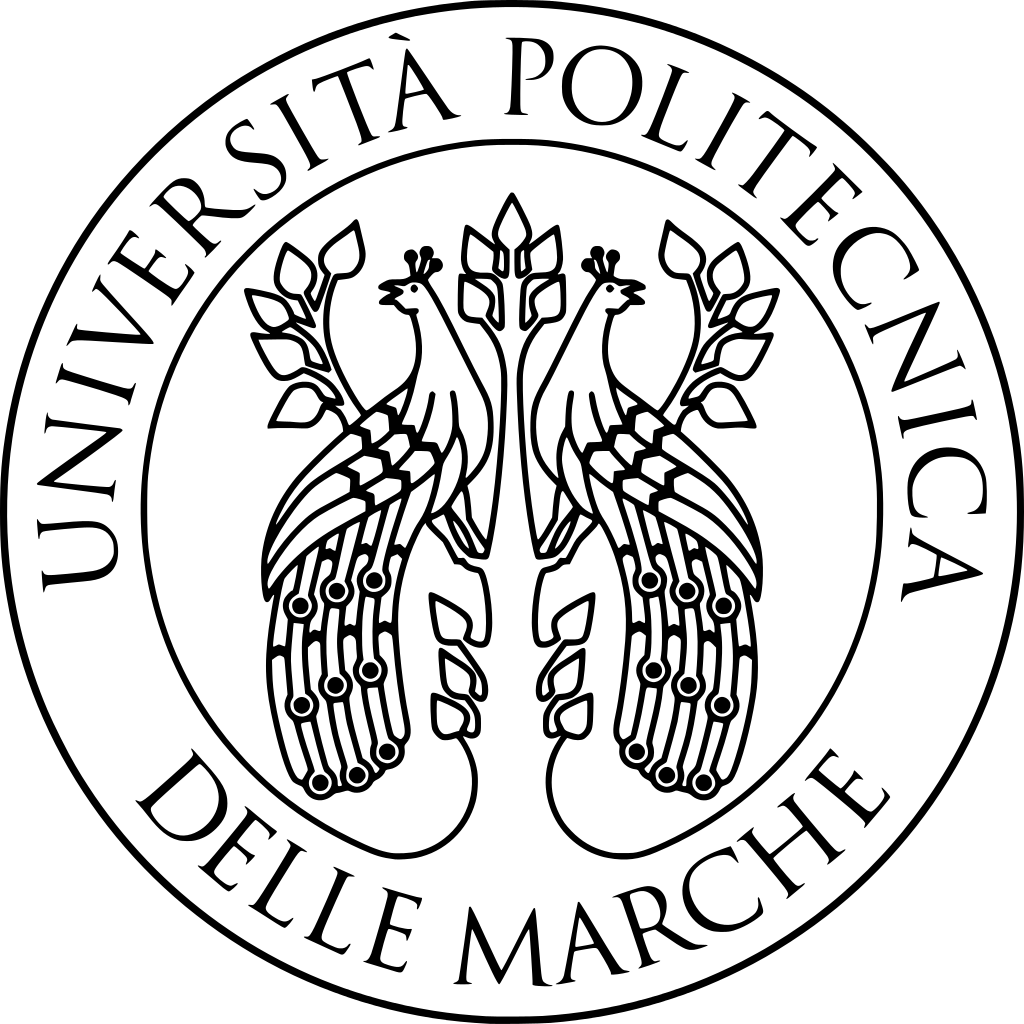
\includegraphics[height=5cm]{figure/logo}\par\vspace{2cm}
\textbf{\Large Titolo in italiano della Tesi di Laurea}\par
\noindent\rule{.3\textwidth}{1pt}\par\vspace{2ex}
\eng{\bfseries\Large Thesis Title in English}\par\vspace{\fill}
{\renewcommand{\arraystretch}{1.2} % righe più spaziate...
\begin{tabular*}{.9\textwidth}{l@{\extracolsep{\fill}}r}
{\large Tesi di Laurea} di: & {\large Relatore}:\\
\textbf{\large Mario Rossi} & \textbf{\large Prof. Aldo Verdi}\\[9ex]
~ & {\large Correlatore}:\\
~ & \textbf{\large Prof. Claudio Bianchi}
\end{tabular*}} % ...solo fino a qui
\vfill\noindent\rule{\textwidth}{1pt}\vspace{2ex}
\textbf{\large Anno Accademico 2016-2017}\par} % parskip 0 finisce qui
\end{center}
\restoregeometry
\clearpage{\pagestyle{empty}\cleardoublepage}
\tableofcontents
\cleardoublepage
\chapter{Ringraziamenti}
Voglio ringraziare\dots{}
\cleardoublepage
\chapter{Sommario}
L'obiettivo di questa Tesi è quello di\dots{}
\clearpage{\pagestyle{empty}\cleardoublepage}

\mainmatter
\pagestyle{fancy}
\chapter{Lorem}
\lipsum[1]
\section{Lorem ipsum}
\lipsum[2-4]
\subsection{Dolor}
\lipsum[5]
\section{Sit amet}
\lipsum[6-8]
Citazione random \cite{lamport82} con nota a piè di pagina\footnote{Nota.}.\par
\lipsum[9]
\clearpage{\pagestyle{plain}\cleardoublepage} % le pagine saltate solo col numero\clearpage{\pagestyle{plain}\cleardoublepage}
\appendix
\chapter{Ipsum}
\section{Sezione}
\lipsum[1-4]\clearpage{\pagestyle{plain}\cleardoublepage}

\backmatter
\pagestyle{plain}\printbibliography[heading=bibintoc] % bibliografia senza testatine
\end{document}